\vspace{-2pt}
\subsection{MAAR Platform Evaluation in DSE}
\label{subsec:res-overall}

\begin{figure}[h]
\vspace{-8pt}
	\centering
		\subfloat[MAAR and DSS] {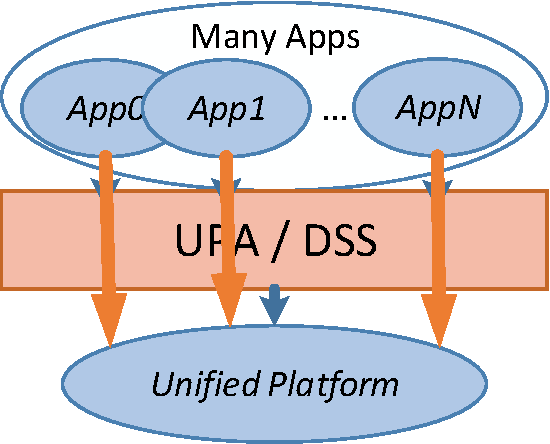
\includegraphics[width=.28\linewidth]{fig/DSSMAAR.pdf}\label{fig:mapMAAR}}
		\hfill
		\subfloat[1appDSE] {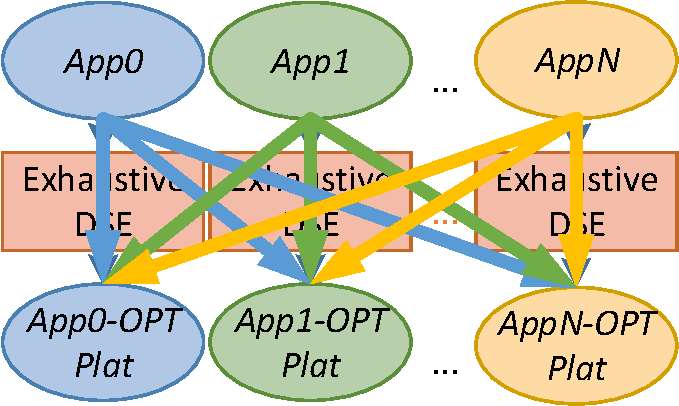
\includegraphics[width=.32\linewidth]{fig/FOP.pdf}\label{fig:mapFOP}}
		\hfill
		\subfloat[OOP] {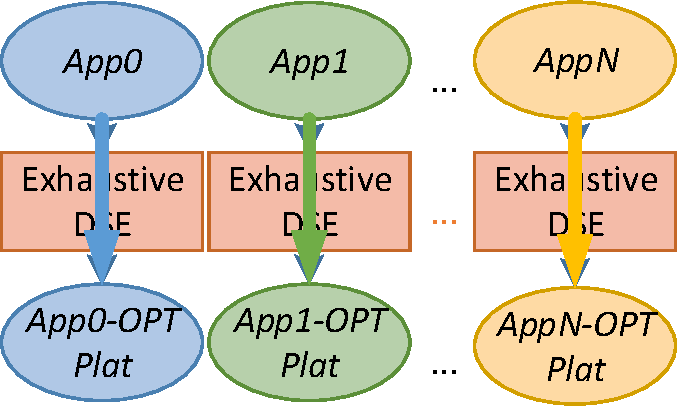
\includegraphics[width=.32\linewidth]{fig/OOP.pdf}\label{fig:mapOOP}}
	\vspace{-8pt}
	\caption{Experiments Settings}
	\label{fig:avg}
\end{figure}

To understand the benefits of MAAR Evaluation, this section compares MAAR DSE with DSS~\cite{zhang2018ds} and 1appDSE. \newtext{As \figref{fig:mapMAAR} shown, both MAAR and DSS platform is designed for many applications. DSS is a greedy algorithm for platform allocation according to characteristics analysis across applications without an evaluation. While in \figref{fig:mapFOP},} 1appDSE considers one application in isolation instead of many applications. In the experiments, an exhaustive search is used to find the 1appDSE platform, which gives the optiamal (OPT) platform for one application. Then mapping all applications on this platform provides one 1appDSE platform performance. To get the average performance of 1appDSE, this paper maps all applications onto all OPT platforms (one platform from one application). Similar to OOP, 1appDSE results in the same number of platforms. However, \newtext{OOP in \figref{fig:mapOOP} only maps the application on its Own Optimal Platform (OOP), while 1appDSE maps all applications onto each platform.}

\newtext{
Next, this paper analyzes the efficiency improvement in Section \ref{subsubsec:overall-sw}, the efficiency achievement in Section \ref{subsubsec:overall-oop} and the number of unique ACCs of different DSE platform(s) in Section \ref{subsubsec:overall-accs}, to show the value of MAAR platform.
}